%
% @author   Shmish  "shmish90@gmail.com"
% @legal    MIT     "(c) Christopher Schmitt"
%


\documentclass{article}


%
% Document Imports
%

\usepackage{fancyhdr}
\usepackage{extramarks}
\usepackage{amsmath}
\usepackage{amssymb}
\usepackage{amsthm}
\usepackage{amsfonts}
\usepackage{color}
\usepackage{tikz}
\usepackage{listings}



%
% Document Configuration
%

\newcommand{\hwAuthor}{Christopher K. Schmitt}
\newcommand{\hwSubject}{CS 483}
\newcommand{\hwSection}{Section 01}
\newcommand{\hwSemester}{Fall 2020}
\newcommand{\hwAssignment}{Assignment 4}

\usetikzlibrary{arrows,automata}
\usetikzlibrary{calc}


%
% Document Environments
%

\setlength{\headheight}{65pt}
\pagestyle{fancy}
\lhead{\hwAuthor}
\rhead{
  \hwSubject \\
  \hwSection \\
  \hwSemester \\
  \hwAssignment
}

\newenvironment{problem}[1]{
  \nobreak\section*{Problem #1}
}{}


%
% Document Start
%

\begin{document}
  \begin{problem}{1}
    $M_1$ = On input string $w$:  \begin{enumerate}
      \item Zig-zag across the tape to corresponding positions on
      either side of the ``\~{}'' symbol.  If the symbols at these
      positions are different ($0 \to 1, 1 \to 0$), check off both
      of these positions.  If the symbols in these positions are the
      same, reject immediately.

      \item When all the symbols to the left of the ``\~{}'' have been
      marked, check for any unchecked symbols to the right of of the
      ``\~{}'' symbol.  If there are any unchecked symbols to the right
      of the ``\~{}'' symbol, reject immediately.  Otherwise accept.
    \end{enumerate}
  \end{problem}

  \begin{problem}{2}
    $M = (A, \Sigma, \Gamma, \delta, q_0, q_9)$
    \begin{center}
      \begin{tikzpicture}[>=stealth',shorten >=1pt,auto,node distance=2.5cm]
        \node[state, initial] (q0) {$q_0$};
        
        \node[state] (q1) [below right of = q0] {$q_1$};
        \node[state] (q2) [right of = q1] {$q_2$};
        
        \node[state] (q3) [above right of = q0] {$q_3$};
        \node[state] (q4) [right of = q3] {$q_4$};

        \node[state] (q5) [above right of = q2] {$q_5$};
        \node[state] (q6) [right of = q5] {$q_6$};

        \node[state] (q7) [above of = q0] {$q_7$};
        \node[state, accepting] (q8) [above of = q7] {$q_8$};

        \path[->] (q0) edge node[right] {$1 \to x, R$} (q3);
        \path[->] (q3) edge node {$\sim \to R$} (q4);
        \path[->] (q4) edge node {$0 \to x, L$} (q5);
        \path[->] (q3) edge[loop above] node {$0, 1 \to R$} (q3);
        \path[->] (q4) edge[loop above] node {$x \to R$} (q4);

        \path[->] (q0) edge node {$0 \to x, R$} (q1);
        \path[->] (q1) edge node {$\sim \to R$} (q2);
        \path[->] (q2) edge node {$1 \to x, L$} (q5);
        \path[->] (q1) edge[loop below] node {$0, 1 \to R$} (q1);
        \path[->] (q2) edge[loop below] node {$x \to R$} (q2);

        \path[->] (q5) edge[loop left] node {$0, 1, x \to L$} (q5);
        \path[->] (q5) edge node {$\sim \to L$} (q6);
        \path[->] (q6) edge[loop above] node {$0, 1 \to L$} (q6);
        \draw[rounded corners, ->] (q6) -- ($(q6) - (0, 4)$) -- ($(q0) - (0, 4)$) node[midway, below] {$x \to R$} -- (q0);

        \path[->] (q0) edge node[left] {$\sim \to R$} (q7); 
        \path[->] (q7) edge[loop left] node {$x \to R$} (q7);
        \path[->] (q7) edge node {$\sqcup \to R$} (q8);
      \end{tikzpicture}
    \end{center}
  \end{problem}

  \pagebreak
  \begin{problem}{3}
    \begin{center}
      \begin{verbatim}
        states = {q0, q1, q2, q3, q4, q5, q6, q7, q8, q9}
        input_alphabet = {0, 1, ~}
        tape_alphabet_extra = {x, _}
        start_state = q0
        accept_state = q8
        reject_state = q9
        num_tapes = 1
        delta =
          q0, 1 -> q3, x, R;
          q0, 0 -> q1, x, R;
          q0, ~ -> q7, ~, R;
          
          q1, 0 -> q1, 0, R;
          q1, 1 -> q1, 1, R;
          q1, ~ -> q2, ~, R;
        
          q2, x -> q2, x, R;
          q2, 1 -> q5, x, L;
        
          q3, 0 -> q3, 0, R;
          q3, 1 -> q3, 1, R;
          q3, ~ -> q4, ~, R;
        
          q4, x -> q4, x, R;
          q4, 0 -> q5, x, L;
        
          q5, 0 -> q5, 0, L;
          q5, 1 -> q5, 1, L;
          q5, x -> q5, x, L;
          q5, ~ -> q6, ~, L;
        
          q6, 0 -> q6, 0, L;
          q6, 1 -> q6, 1, L;
          q6, x -> q0, x, R;
        
          q7, x -> q7, x, R;
          q7, _ -> q8, _, R;
      \end{verbatim}

      \includegraphics[scale=0.5]{images/0.jpg}
      \includegraphics[scale=0.5]{images/1.jpg}
      \includegraphics[scale=0.5]{images/2.jpg}
      \includegraphics[scale=0.5]{images/3.jpg}
      \includegraphics[scale=0.5]{images/4.jpg}
      \includegraphics[scale=0.5]{images/5.jpg}
      \includegraphics[scale=0.5]{images/6.jpg}
      \includegraphics[scale=0.5]{images/7.jpg}
      \includegraphics[scale=0.5]{images/8.jpg}
      \includegraphics[scale=0.5]{images/9.jpg}
      \includegraphics[scale=0.5]{images/10.jpg}
      \includegraphics[scale=0.5]{images/11.jpg}
      \includegraphics[scale=0.5]{images/12.jpg}
      \includegraphics[scale=0.5]{images/13.jpg}
      \includegraphics[scale=0.5]{images/14.jpg}
      \includegraphics[scale=0.5]{images/15.jpg}
      \includegraphics[scale=0.5]{images/16.jpg}
      \includegraphics[scale=0.5]{images/17.jpg}
      \includegraphics[scale=0.5]{images/18.jpg}
    \end{center}
  \end{problem}

  \begin{problem}{4}
    \begin{proof}
      $ $\newline
      Let $M_1$ be a Turing machine which decides $L_1$
      
      \noindent
      Let $M_2$ be a Turing machine which decides $L_2$

      \noindent
      We can define $M_3$, the Turing machine which decides
      $L_1 \cap L_2$, like so:

      \begin{center}
        $M_3$ = On input string $w$: \begin{enumerate}
          \item Run both $M_1$ and $M_2$, one right after the other
          \item If $M_1$ accepts $w$ and $M_2$ accepts $w$, accept $w$
          \item If either $M_1$ or $M_2$ reject $w$, reject $w$
        \end{enumerate}
      \end{center}

      \noindent
      $M_3$ accepts when $w \in L_1 \cap L_2$ and rejects when
      $w \notin L_1 \cap L_2$.  Because $M_1$ and $M_2$ are
      gaurenteed to halt ($L_1$ and $L_2$ are decidable), $M_3$ is
      also gaurenteed to halt.  Therefore, $L_1 \cap L_2$ is
      decidable.
      
      $ $\newline
    \end{proof}
  \end{problem}

  \pagebreak

  \begin{problem}{5}
    \begin{proof}
      $ $\newline
      Let $M_1$ be a Turing machine which decides $L_1$

      \noindent
      Let $M_2$ be a Turing machine which decides $L_2$

      \noindent
      We can define $M_3$, the Turing machine which decides
      $L_1L_2$, like so:

      \begin{center}
        $M_3$ = On input string $w$: \begin{enumerate}
          \item Split the string $w$ into two parts, $LHS$ and $RHS$
          \item Run $M_1$ on $LHS$ and $M_2$ on $RHS$.
          \item If $M_1$ accepts $LHS$ and $M_2$ accepts $RHS$, accept $w$
          \item If Either $M_1$ or $M_2$ reject, return to step one and shift the split position to the right by one.  If this goes beyond the end of $w$, reject.
        \end{enumerate}
      \end{center}

      \noindent
      $M_3$ accepts when $w \in L_1L_2$ and rejects when
      $w \notin L_1L_2$.  Because $M_1$ and $M_2$ are
      gaurenteed to halt ($L_1$ and $L_2$ are decidable), $M_3$ is
      also gaurenteed to halt.  Therefore, $L_1L_2$ is
      decidable.

      $ $\newline
    \end{proof}
  \end{problem}

  \begin{problem}{6}
    \begin{proof}
      $ $\newline
      Let $M_1$ be a Turing machine which recognizes $L_1$

      \noindent
      Let $M_2$ be a Turing machine which recognizes $L_2$

      \noindent
      We can define $M_3$, the Turing machine which recognizes
      $L_1 \cap L_2$, like so:

      \begin{center}
        $M_3$ = On input string $w$: \begin{enumerate}
          \item Run both $M_1$ and $M_2$, one right after the other
          \item If $M_1$ accepts $w$ and $M_2$ accepts $w$, accept $w$
          \item If either $M_1$ or $M_2$ reject $w$, reject $w$
          \item If $M_1$ loops, then $M_3$ is also looping ($M_3$ runs $M_1$)
          \item If $M_2$ loops, then $M_3$ is also looping ($M_3$ runs $M_2$)
        \end{enumerate}
      \end{center}

      \noindent
      $M_3$ accepts when $w \in L_1 \cap L_2$ and rejects (or loops)
      when $w \notin L_1 \cap L_2$.  Because $M_1$ and $M_2$ are
      gaurenteed to accept, reject, or loop ($L_1$ and $L_2$ are 
      recognizable), $M_3$ is also gaurenteed to accept, reject, or 
      loop.  Therefore, $L_1 \cap L_2$ is recognizable.

      $ $\newline
    \end{proof}
  \end{problem}

  \begin{problem}{7}
    \begin{proof}
      $ $\newline
      Let $M_1$ be a Turing machine which recognizes $L_1$

      \noindent
      Let $M_2$ be a Turing machine which recognizes $L_2$

      \noindent
      We can define $M_3$, the Turing machine which recognizes
      $L_1L_2$, like so:

      \begin{center}
        $M_3$ = On input string $w$: \begin{enumerate}
          \item Split the string $w$ into two parts, $LHS$ and $RHS$
          \item Run $M_1$ on $LHS$ and $M_2$ on $RHS$.
          \item If $M_1$ accepts $LHS$ and $M_2$ accepts $RHS$, accept $w$
          \item If Either $M_1$ or $M_2$ reject, return to step one and shift the split position to the right by one.  If this goes beyond the end of $w$, reject.
        \end{enumerate}
      \end{center}

      \noindent
      $M_3$ accepts when $w \in L_1L_2$ and rejects or loops when
      $w \notin L_1L_2$.  Because $M_1$ and $M_2$ are
      gaurenteed to accept or loop ($L_1$ and $L_2$ are recognizable), $M_3$ is
      also gaurenteed to halt or loop.  Therefore, $L_1L_2$ is
      recognizable.

      $ $\newline
    \end{proof}
  \end{problem}

  \begin{problem}{8}
    \begin{proof}
      $ $\newline
      If $L(A) = \Sigma^*$, then every state of $A$ must be an
      accepting state.  For each state in $A$, check to see if
      it is an accepting state.  If it is not, then reject.  If
      all states are accepting, accept.  Because a DFA has a
      finite number of states, the machine will always halt, so
      this language is decidable.

      $ $\newline
    \end{proof}
  \end{problem}

  \begin{problem}{9}
    \begin{proof}
      $ $\newline
      The language is decidable.  Construct a machine which performs
      the following operations.

      \begin{enumerate}
        \item Convert $R$ to an NFA, $R'$
        \item Convert $R'$ to a DFA, $R''$
        \item Construct a new DFA, $R_\Delta$, which accepts the symmetric difference of $L(D)$ and $L(R'')$
        \item If the language of $R_\Delta$ is $\emptyset$, then accept, otherwise reject.  Note that it is sufficent to check weather there are any paths to an accepting state to determine this.
      \end{enumerate}
    \end{proof}
  \end{problem}
\end{document}